\documentclass[12pt]{article}

\usepackage{hyperref}
\usepackage[english]{babel}
\usepackage[letterpaper]{geometry}
\usepackage{amsmath}
\usepackage{amssymb}
\usepackage{amsfonts}
\usepackage{graphicx}

\author{Mart\'{\i}nez Gonz\'alez, Gabriel}
\date{\today}
\title{Tarea 3: Proyecto (factorizaci\'on de n\'umeros primos)}

\begin{document}
\maketitle
\begin{abstract}

	En el documento se explicará el algoritmo mate\'atico \textit{divisi\'on por tentativa} para averiguar si un n\'unmero es primo o no, adem\'as de su implementaci\'on y como, a partir de esto, conocer la factorizaci\'on en n\'umeros primos de cualquier entero positivo.

\end{abstract}

\section{Teor\'{i}a detr\'as del algoritmo}

Sea $n$ un n\'umero entero positivo. Tenemos que, si es compuesto, podemos hacer el siguiente razonamiento:\\
Si $n mod 2=0$, entonces 2 es factor de $n$ por definici\'on. M\'as a\'un, podemos darnos cuenta que $\frac{n}{2}$ es el factor m\'as grande (no necesariamente primo) que podría tener $n$, pues 
$$\frac{n}{2}\cdot 2=n$$
y por otro lado
$$\left(\frac{n}{2} +1\right)\cdot 2>n$$
\\
Dado este hecho, podemos darnos cuenta que, si 2 es factor, s\'olo basta comprobar los n\'umeros menores o iguales que $\frac{n}{2}$ para encontrar el resto de factores de $n$. Pero incluso si 2 no es factor, el mismo principio sigue funcionando, pues de haberlo sido, $\frac{n}{2}$ habría sido el factor m\'as grande, por lo que el resto de factores tendr\'{i}an que estar (y de hecho, lo est\'an) por debajo de este umbral.  
As\'{i} pues, tenemos que este proceso lo podemos realizar con cualquier n\'umero primo menor que $n$. Por lo que, si aplicamos reiteradamente el proceso, el n\'umero primo mayor al que podemos aspirar a llegar (suponiendo que ninguno menor haya sido factor) es
$$\sqrt{n}$$
Ya que $(\sqrt{n})^2=n$

Observemos que no estamos diciendo que $\sqrt{n}$ sea un factor primo de $n$ (es m\'as, muchas veces este n\'umero ser\'a real y no entero); pues este es el caso en el que ning\'uno de los otros n\'umeros primos menores a $\sqrt{n}$ sean factores de $n$. Pero, aplicando nuevamente uno de los hechos que señalamos anteriormente, si existe un factor de $n$, este tendr\'{i}a que ser menor o igual a la ra\'{i}z de $n$.

Entonces, dado todo este preambulo, podemos darnos cuenta que, simplemente, tenemos que fijarnos en los n\'umeros menores o iguales que $\sqrt{n}$ para encontrar un factor de $n$ y determinar si es primo o no. Es en este punto en el que se ha optimizado el algoritmo de fuerza bruta, tal que para $n=100$, s\'olo har\'{i}an falta 10 comprobaciones (y no las 100 que ser\'{i}an por fuerza bruta); menos a\'un, tomando en cuenta que no se analiza el propio 1.

Ahora bien, señalemos el siguiente ejemplo:
$$n=35$$
Nos damos cuenta que $\sqrt{n}<6$, pero $7\cdot 5=35$. Esto sucede porque el m\'etodo construido s\'olo asegura encontrar un factor por debajo de la cota, no encontrarlos todos. Sin embargo, es facil darnos cuenta que si tenemos un n\'umero primo factor de $n$, $p$, que satisfaga $p>\sqrt{n}$, siempre se puede encontrar el n\'umero $r$, tal que:
$$r\cdot p = n$$
En la practica vemos que $r=\frac{n}{p}$ y que no tiene por qu\'e ser primo. Observemos que:
$$p>\sqrt{n}\Longrightarrow p\cdot\sqrt{n}>n\Longrightarrow \sqrt{n}>\frac{n}{p}$$
Tambi\'en cabe señalar que, este mismo analis\'{i}s es valido si intercambiamos que $r$ sea primo y $p$ no necesariamente.

As\'i pues, podemos darnos cuenta que para obtener todos los factores primos de $n$, se pueden comprobar todos los n\'umeros menores que $\sqrt{n}$ y, en caso de encontrarse un primo, comprobar la existencia de un factor mayor a $\sqrt{n}$ y, nuevamente, corroborar si es primo o compuesto con el mismo m\'etodo.

\section{Implementaci\'on en c\'odigo}

El c\'odigo que se ha implementado se divide en cuatro partes, las cuales llamaremos \textit{main}, \textit{comprobar}, \textit{cota}, \textit{multiplicidad}.

\subsection{main}
\begin{center}
 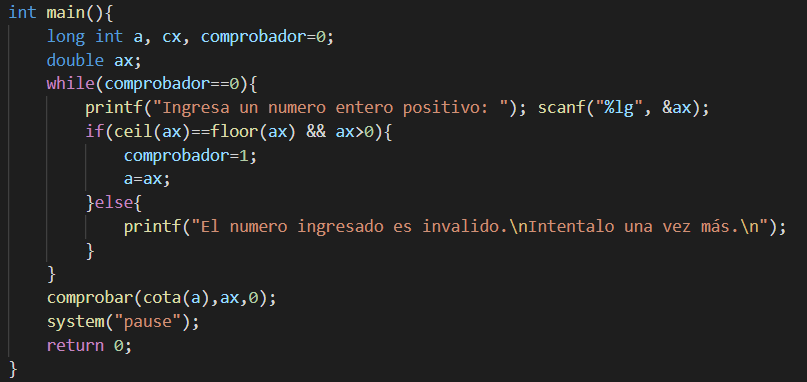
\includegraphics[scale=0.9]{main}
\end{center}

En esta secci\'on, simplemente, se implemento un comprobador para determinar si el n\'umero ingresado es entero positivo. Así mismo, se llama a las funciones que implementar\'an el algoritmo descrito anteriormente.

\subsection{cota}
\begin{center}
 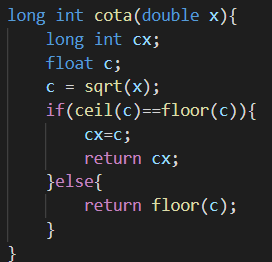
\includegraphics[scale=1]{cota}
\end{center}

Esta funci\'on simplemente calcular\'a la ra\'{i}z del n\'umero por analizar, as\'{i} como determinar si dicha ra\'{i}z es real o entera y en caso de ser real, devolver\'a el valor techo de dicho n\'umero (para evitar descartar un candidato valido).

\subsection{comprobar}
\begin{center}
 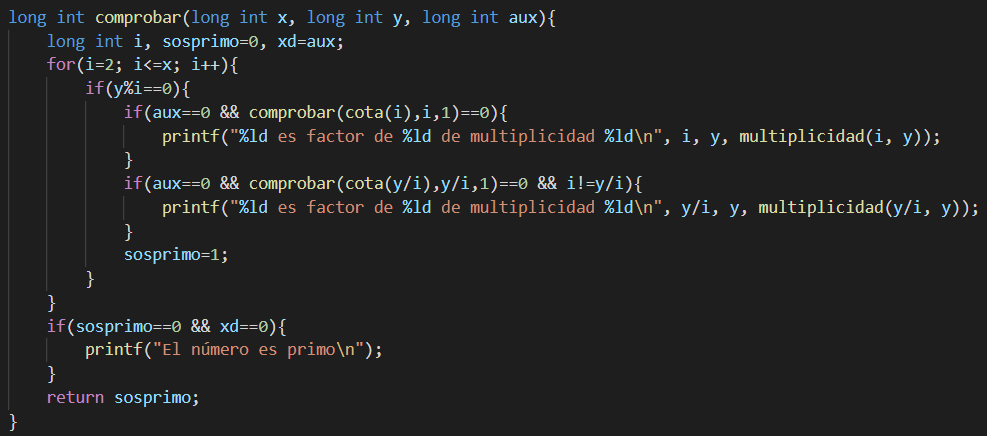
\includegraphics[scale=0.7]{comprobar}
\end{center}

Este es el fragmento de c\'odigo que, realmente, implementa todo lo que se describio anteriormente, donde se piden tres entradas: la cota calculada con la funci\'on anterior, el n\'umero a analizar y una entrada que servir\'a para realizar las comprobaciones de si el factor que se analiza es primo o no, pero sin imprimir informaci\'on que haga ruido.
Se implementa el ciclo que, normalmente, har\'{i}a la fuerza bruta. Pero en este caso s\'olo llegando a la cota prefijada. As\'{i} pues, para cada n\'umero, posible factor, a analizar, se comprueba si es primo o no llamando a la misma funci\'on, s\'olo cambiando los argumentos. Hay que aseverar que, el \textit{if} que analiza si son primos o no tiene la propiedad de que s\'olo se entrar\'a en \'el si el n\'umero en cuesti\'on no es primo. De ah\'{i} que se busque que, al entrar en el \textit{if}, una variable cambie para determinar que no puede ser primo; y en caso de quedar inalterada, se determine que el n\'umero s\'olo puede ser primo.
As\'i mismo, se señala que hay una variable auxiliar que sirve para evitar imprimir cualquier tipo de informaci\'on al analizar los factores del n\'umero ingresado por el usuario. 

\subsection{multiplicidad}
\begin{center}
 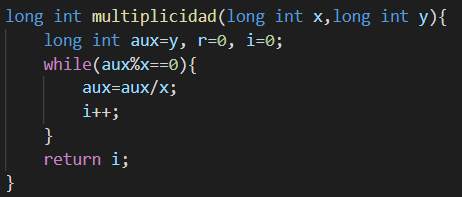
\includegraphics[scale=1]{multiplicidad}
\end{center}

Dado que la funci\'on de comprobaci\'on solo puede decir si un factor es primo o no, la funci\'on multiplicidad busca que, cuando se compruebe que un n\'umero s\'{i} es primo, cuente cuantas veces este n\'umero divide al ingresado por el usuario y de ah\'i obtener su multiplicidad. 

\end{document}